\documentclass[a4paper, 11pt, oneside]{report}

%----------------------------------------------------------------------------------------
% Placeholders — replace before final submission
%----------------------------------------------------------------------------------------
\newcommand{\ProjectTitle}{InsightHR}
\newcommand{\ProjectSubtitle}{Intelligent Employee Management \& Decision Support System}
\newcommand{\ProjectCertificateTitle}{InsightHR: Intelligent Employee Management \& Decision Support System}
\newcommand{\StudentName}{Your Name}
\newcommand{\StudentRoll}{2201xxxx}
\newcommand{\StudentSemester}{VI}
\newcommand{\StudentEmail}{xxxx@iiitmanipur.ac.in}
\newcommand{\SupervisorName}{Dr.\,........}
\newcommand{\SupervisorDesignation}{Supervisor Designation}
\newcommand{\SupervisorPhone}{+91\,xxxxxxxxx}
\newcommand{\SupervisorEmail}{supervisor@iiitmanipur.ac.in}
\newcommand{\ReportMonthYear}{April, 2026}
\newcommand{\DeclarationDate}{DD-MM-YYYY}

\newcommand{\plogo}{\fbox{$\mathcal{PL}$}}
\usepackage{graphicx}
\usepackage{float}
\usepackage[table,xcdraw]{xcolor}
\usepackage[utf8]{inputenc}
\usepackage[T1]{fontenc}
\usepackage{fouriernc}
\usepackage{subcaption}
\usepackage{tikz}
\usepackage{pgfplots}
\usepackage{longtable}
\usepackage[nottoc]{tocbibind}
\usepackage{url}
\usepackage{amsmath}
\usepackage{booktabs}
\usepackage{listings}
\lstset{
  basicstyle=\ttfamily\small,
  breaklines=true,
  frame=single,
  tabsize=2
}
\usepackage{hyperref}
\hypersetup{colorlinks=true, linkcolor=blue, urlcolor=blue, citecolor=blue}
% \usepackage{lipsum} % uncomment for dummy text

\begin{document}

\begin{titlepage}
  \centering
  \vspace*{\baselineskip}
  \vspace{0.75\baselineskip}
  {\Huge \bfseries \ProjectTitle}\\[0.6\baselineskip]
  {\large \ProjectSubtitle}
  \vspace{0.75\baselineskip}
  \vspace{2\baselineskip}
  A report submitted for the course named Project - I (CS3201)
  \vspace*{7\baselineskip}
  Submitted By
  \vspace{0.5\baselineskip}
  {\scshape\Large \StudentName \\ \StudentSemester \\ \StudentRoll}
  \vspace{0.5\baselineskip}
  Supervised By
  \vspace{0.5\baselineskip}
  {\scshape\Large \SupervisorName}
  \vspace{0.5\baselineskip}
  \vfill
  \begin{center}
    \IfFileExists{report_file/iiit_manipur.png}{%
      \includegraphics[width=5cm]{report_file/iiit_manipur.png}%
    }{%
      \fbox{\parbox[c][3cm][c]{5cm}{\centering \small [Place institute logo:\\ \texttt{report\_file/iiit\_manipur.png}]}}%
    }
  \end{center}
  {\scshape\small Department of Computer Science and Engineering\\ Indian Institute of Information Technology Senapati, Manipur \\ \ReportMonthYear}
\end{titlepage}

%----------------------------------------------------------------------------------------
% Declaration
%----------------------------------------------------------------------------------------
\begin{center}
  {\LARGE \textbf{Declaration}}
\end{center}
In this submission, I have expressed my idea in my own words, and I have adequately cited and referenced any ideas or words that were taken from another source. I also declare that I adhere to all principles of academic honesty and integrity and that I have not misrepresented or falsified any ideas, data, facts, or sources in this submission. If any violation of the above is made, I understand that the institute may take disciplinary action. Such a violation may also engender disciplinary action from the sources which were not properly cited or permission not taken when needed.

\vspace{1cm}\hspace{8.35cm} \StudentName \\
\vspace{1cm}\hspace{9cm} \StudentRoll \\
\vspace{1cm} DATE: \DeclarationDate

\newpage

%----------------------------------------------------------------------------------------
% Certificate (bonafide)
%----------------------------------------------------------------------------------------
\begin{center}
  \thispagestyle{empty}
  \begin{table}
    \centering
    \IfFileExists{report_file/iiit_manipur.png}{%
      \includegraphics[scale=0.2]{report_file/iiit_manipur.png}%
    }{%
      \fbox{\small Logo placeholder}%
    }
    \begin{tabular}{l}
      Department of Computer Science and Engineering \\
      Indian Institute of Information Technology Senapati, Manipur \\
    \end{tabular}
  \end{table}
  \par\noindent\rule{\textwidth}{0.4pt}
  \SupervisorName
  \hspace*{\fill} Email: \href{mailto:\SupervisorEmail}{\SupervisorEmail}\\
  \SupervisorDesignation
  \hspace*{0pt}\hfill Contact No: \SupervisorPhone\\[2cm]
  {\Huge \textbf{\emph{To Whom It May Concern}}}\\[2cm]
  \linespread{1.13}
  \large This is to certify that the project report entitled \textbf{``\ProjectCertificateTitle,''} submitted to the department of Computer Science and Engineering, Indian Institute of Information Technology Senapati, Manipur in partial fulfilment for the award of degree of Bachelor of Technology in Computer Science and Engineering is bona fide work carried out by \textbf{\StudentName} bearing roll number \StudentRoll.\\[2.0cm]
  \hspace*{2.6in}\large{Signature of Supervisor}\\[0.3cm]
  \hspace*{2.5in}\textbf{(\SupervisorName)}\\[0.5cm]
\end{center}
\vspace{0.5cm}
Signature of the Examiner 1 \dotfill\\[0.5cm]
Signature of the Examiner 2 \dotfill\\[0.5cm]
Signature of the Examiner 3 \dotfill\\[0.5cm]
Signature of the Examiner 4 \dotfill\\
\newpage

%----------------------------------------------------------------------------------------
% Abstract
%----------------------------------------------------------------------------------------
\begin{abstract}
Modern organisations need more than static employee records: they require \emph{decision support}---transparent scoring, workload-aware task assignment, and early signals for attrition or promotion readiness. This project presents \textbf{InsightHR}---an \textbf{Intelligent Employee Management \& Decision Support System}: a full-stack web application that combines role-based access, CRUD operations for employees and tasks, and \textbf{explainable analytics}. Performance is computed using a configurable weighted model over attendance, task completion, deadline adherence, and peer feedback, with stored breakdowns for audit and trend visualisation. A \textbf{smart task allocation} module ranks candidates using skill overlap, availability, and workload penalties, returning top recommendations with natural-language justifications. \textbf{Attrition risk}, \textbf{anomaly detection} (statistical and rule-based), and \textbf{promotion recommendations} are implemented as lightweight, interpretable engines suitable for demonstration and extension toward machine learning. The stack uses React (Vite), Tailwind/ShadCN-style UI, Node.js/Express, MongoDB, JWT with HTTP-only cookies, and optional Google OAuth~2.0. The outcome is a demo-ready system aligned with software engineering practice: validation, error handling, modular services, and report-oriented APIs.
\end{abstract}
\pagebreak

%----------------------------------------------------------------------------------------
% Acknowledgement
%----------------------------------------------------------------------------------------
\begin{center}
  {\LARGE \textbf{Acknowledgement}}
\end{center}
\vspace{1cm}
I express sincere gratitude to my supervisor, \SupervisorName, for guidance, feedback, and encouragement throughout this project. I thank the faculty of the Department of Computer Science and Engineering, IIIT Manipur, for foundational courses that enabled this work. I acknowledge open-source communities whose frameworks and libraries accelerated development. Finally, I thank my family and peers for their support.

\vspace{1.5cm}
\hspace{7cm} \StudentName\\
\hspace{7cm} Roll: \StudentRoll

\newpage

\tableofcontents
\listoffigures
\listoftables

\chapter{Introduction}
\section{Background}
\textbf{InsightHR} is the working title of the software developed in this project: an intelligent employee management platform with embedded decision-support analytics. Human-resource (HR) and people-operations teams increasingly rely on digital systems to maintain employee master data, track performance, and coordinate work. Traditional \emph{employee portals} often reduce to create--read--update--delete (CRUD) screens with limited analytical depth. In contrast, a \textbf{decision support system (DSS)} aims to structure data, models, and explanations so managers can interpret recommendations rather than only viewing raw tables \cite{power2002}.

\section{Problem Statement}
Organisations face recurring questions: \emph{Who should receive the next critical task given skills and current load?} \emph{Which employees show early signals of disengagement or attrition?} \emph{How can performance be summarised fairly and explained to staff?} \emph{Who merits promotion discussion based on consistent evidence?} Answering these questions with spreadsheets alone is error-prone and weakly auditable. There is a need for an integrated system that (i)~unifies identity and authorisation, (ii)~maintains authoritative employee and task records, and (iii)~exposes \textbf{interpretable} analytics aligned with organisational policy (e.g.\ configurable weights).

\section{Objectives}
The primary objectives of this project are:
\begin{itemize}
  \item To design and implement a secure, role-based web application for employee and task management.
  \item To provide a \textbf{performance scoring engine} with configurable weights and stored factor breakdowns for transparency.
  \item To implement \textbf{smart task allocation} that ranks employees using skill match, availability, and workload penalties, with textual explanations.
  \item To deliver \textbf{attrition risk estimation}, \textbf{anomaly detection} on performance history, and \textbf{promotion recommendations} using lightweight, explainable logic suitable for academic demonstration and future ML extension.
  \item To present information through \textbf{role-specific dashboards} with charts and alerts for operational review.
\end{itemize}

\section{Scope}
\textbf{In scope:} authentication (email/password and optional Google OAuth~2.0), JWT sessions via HTTP-only cookies, MongoDB persistence, REST APIs, React single-page client, seed data for demonstration, and documented analytics semantics.

\textbf{Out of scope (explicit):} payroll processing, legal compliance certification, production-scale ML training pipelines, and integration with third-party HRIS beyond illustrative API design. Analytics are \textbf{rule-based and statistical} with clear labelling; they support decision support but are not a substitute for human judgement.

\section{Report Organisation}
Chapter~2 reviews related work. Chapter~3 captures requirements. Chapter~4 presents architecture and design. Chapter~5 describes implementation. Chapter~6 discusses results and testing. Chapter~7 concludes with limitations and future work.


\chapter{Literature Survey}
\section{Decision Support and HR Analytics}
Decision support systems combine data models, analytical components, and presentation layers to assist semi-structured decisions \cite{power2002}. In people analytics, industry and research emphasise \emph{fairness}, \emph{interpretability}, and \emph{governance}: scores and flags should be explainable to employees and regulators where applicable \cite{barocas2019,deloitte2018people}.

\section{Performance Management}
Weighted composite scores are widely used to aggregate multiple KPIs (e.g.\ attendance, delivery, quality). Normalisation and explicit weights improve perceived fairness compared to opaque single numbers. Storing \textbf{breakdowns} alongside aggregates supports audits and trend analysis---a practice aligned with explainable reporting.

\section{Workforce Planning and Task Assignment}
Assignment problems can be framed as matching tasks to agents under capacity constraints. While integer programming and advanced solvers apply at scale, \textbf{heuristic scoring} (skills $+$ capacity $+$ penalty) offers a transparent baseline that communicates trade-offs to users---valuable in educational and pilot deployments.

\section{Attrition and Retention}
Attrition modelling ranges from survival analysis and gradient boosting to simple rule engines driven by domain thresholds (attendance drops, workload spikes, compensation equity). For a capstone prototype, \textbf{rule-based} models with documented factors preserve clarity and map cleanly to later supervised learning while data volume is limited.

\section{Anomaly Detection}
Univariate and multivariate anomaly detection includes z-scores, control charts, and isolation forests. For time series of performance metrics, comparing the latest observation to a local mean with a dispersion estimate (z-score style) is a classical, interpretable approach \cite{chandola2009}.

\section{Gap Addressed by This Project}
Many student projects stop at CRUD. This work contributes an \textbf{integrated} stack where each analytical output is paired with \textbf{explanation text} and \textbf{structured breakdowns}, and where administrative policy (weights) is first-class---bridging HR operations and transparent decision support.


\chapter{Requirement Engineering}
\section{Stakeholders}
\begin{itemize}
  \item \textbf{Administrator:} full configuration, employee lifecycle, analytics oversight, weight settings.
  \item \textbf{Manager:} team tasks, allocation, performance runs, attrition/promotion views, alerts.
  \item \textbf{Employee:} personal dashboard, assigned tasks, own performance history, personal alerts.
\end{itemize}

\section{Functional Requirements}
\subsection{Authentication and Authorisation}
\begin{itemize}
  \item Register and login with email/password; password hashing (bcrypt).
  \item Optional Google OAuth~2.0 via Passport.js; JWT issued after success.
  \item JWT delivered as HTTP-only cookie (Bearer token optional); logout clears session.
  \item Role-based access control on API routes and UI navigation.
\end{itemize}

\subsection{Employee Management}
\begin{itemize}
  \item CRUD for employee profiles: department, designation, skills array, compensation and HR metrics, status, reporting manager, optional link to user account.
  \item Validation: email format, numeric fields, non-empty required strings, valid references.
\end{itemize}

\subsection{Task Management}
\begin{itemize}
  \item CRUD for tasks: title, description, required skills, priority, deadline, estimated hours, status.
  \item Assignment to one employee; guard against accidental double assignment without explicit override.
  \item Recommendation endpoint returning top three candidates with scores and explanations; optional auto-assign.
\end{itemize}

\subsection{Performance Scoring}
\begin{itemize}
  \item Weighted score: $P = w_1 A + w_2 T + w_3 D + w_4 F$ with inputs normalised to $[0,100]$ and weights summing to~1 after normalisation.
  \item Admin-configurable weights; persist breakdown and narrative explanation per calculation.
  \item Trend and history APIs for charting.
\end{itemize}

\subsection{Analytics Modules}
\begin{itemize}
  \item \textbf{Attrition:} risk band, score, reasons, recommended actions, method label.
  \item \textbf{Anomaly:} type, severity, reason, suggested action, explanation; statistical/rule hybrid.
  \item \textbf{Promotion:} ranked candidates with scores and per-candidate explanations.
\end{itemize}

\subsection{Alerts and Dashboards}
\begin{itemize}
  \item Persist alerts (types: anomaly, attrition, performance-drop, promotion); list and mark-read.
  \item Dashboards: aggregates, charts (e.g.\ workload, risk, task mix), recent alerts.
\end{itemize}

\section{Non-Functional Requirements}
\begin{itemize}
  \item \textbf{Security:} Helmet, CORS with credentials, input validation, no sensitive data in client storage for JWT cookie flow.
  \item \textbf{Usability:} responsive layout, loading states, toasts, form validation messages.
  \item \textbf{Maintainability:} modular server layers (routes, controllers, services, models); componentised UI.
  \item \textbf{Demonstrability:} seed script with realistic users, employees, tasks, performance records, and alerts.
\end{itemize}

\section{Constraints}
MongoDB availability; Google OAuth requires developer console configuration; browser third-party cookie policies do not affect same API host with credentialed XHR to backend origin.

\begin{table}[H]
  \centering
  \caption{High-level requirement traceability (summary).}
  \label{tab:req-trace}
  \begin{tabular}{p{3.2cm}p{9cm}}
    \toprule
    \textbf{Theme} & \textbf{Mapped deliverables} \\
    \midrule
    Security & JWT cookie sessions, bcrypt, Helmet/CORS, RBAC middleware \\
    Data model & Mongoose schemas for users, employees, tasks, performance, alerts, settings \\
    Explainability & Breakdown objects, \texttt{explanation}/\texttt{method} fields on analytics responses \\
    UX & Dashboards, validation, toasts, responsive layout \\
    \bottomrule
  \end{tabular}
\end{table}


\chapter{System Design}
\section{High-Level Architecture}
The system follows a \textbf{client--server} pattern with a document database:
\begin{itemize}
  \item \textbf{Client:} React (Vite), Tailwind CSS, ShadCN-style components, React Router, React Hook Form + Zod, Axios (withCredentials), Zustand, Recharts.
  \item \textbf{Server:} Node.js, Express.js, Mongoose, Passport (Google), JWT, bcrypt, Helmet, CORS, Morgan, cookie-parser.
  \item \textbf{Database:} MongoDB collections for users, employees, tasks, performance records, alerts, application settings.
\end{itemize}

\begin{figure}[H]
  \centering
  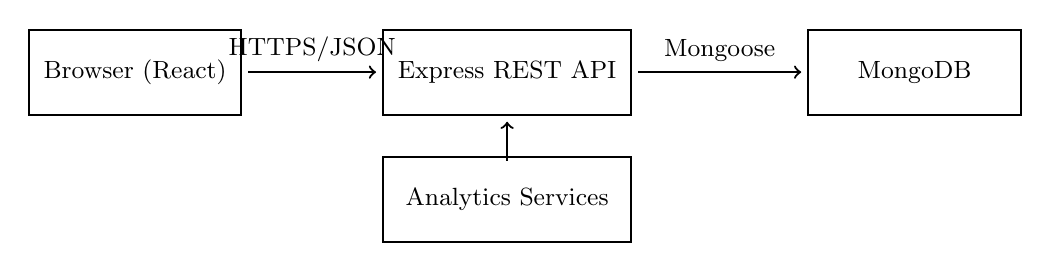
\begin{tikzpicture}[scale=0.9, every node/.style={font=\small}]
    \draw[thick] (0,0) rectangle (3,1.2) node[midway] {Browser (React)};
    \draw[thick] (5,0) rectangle (8.5,1.2) node[midway] {Express REST API};
    \draw[thick] (11,0) rectangle (14,1.2) node[midway] {MongoDB};
    \draw[->, thick] (3.1,0.6) -- node[above] {HTTPS/JSON} (4.9,0.6);
    \draw[->, thick] (8.6,0.6) -- node[above] {Mongoose} (10.9,0.6);
    \draw[thick] (5,-1.8) rectangle (8.5,-0.6) node[midway] {Analytics Services};
    \draw[->, thick] (6.75,-0.65) -- (6.75,-0.1);
  \end{tikzpicture}
  \caption{Logical deployment view (conceptual).}
  \label{fig:arch}
\end{figure}

\section{Data Model (Summary)}
Key entities:
\begin{itemize}
  \item \textbf{User:} identity, credential or Google id, role (\texttt{admin}|\texttt{manager}|\texttt{employee}).
  \item \textbf{Employee:} HR profile, skill tags, operational metrics, embedded performance history snapshots, cached attrition/promotion fields.
  \item \textbf{Task:} specification, required skills, lifecycle status, single assignee reference.
  \item \textbf{PerformanceRecord:} dimensional scores, weighted aggregate, embedded breakdown and explanation.
  \item \textbf{Alert:} typed message with severity and read flag.
  \item \textbf{AppSettings:} global performance weights.
\end{itemize}

\section{Control Flow --- Authentication}
Registration/login validates input, hashes passwords, signs JWT with server secret, sets HTTP-only cookie, and exposes \texttt{/api/auth/me} for session bootstrap. Google OAuth redirects through Passport; on success the same cookie issuance path executes.

\section{Control Flow --- Analytics}
Controllers delegate to \textbf{service modules}: performance engine, task allocation, attrition, anomaly, promotion. Services return JSON including \texttt{explanation} and/or \texttt{method} fields for UI and reporting. This separation keeps routes thin and enables unit-style reasoning about formulas.

\section{API Design}
RESTful resources under \texttt{/api/}: \texttt{auth}, \texttt{employees}, \texttt{tasks} (including \texttt{assign} and \texttt{recommend}), \texttt{performance}, \texttt{ml} (attrition, anomaly, promotion, task-match), \texttt{alerts}, \texttt{settings}. Errors return JSON with clear messages; validation failures list field issues.

\section{Security Design}
Role checks applied after authentication middleware. Employees are scoped to linked profiles for self-service routes. CORS restricted to configured client origin with credentials enabled. Passwords never returned from API; JWT not exposed to JavaScript when using HTTP-only cookies.


\chapter{Implementation}
\section{Repository Structure}
The implementation resides in a monorepo-style layout:
\begin{itemize}
  \item \texttt{client/} --- Vite React application (\texttt{src/pages}, \texttt{components}, \texttt{layouts}, \texttt{services}, \texttt{store}).
  \item \texttt{server/} --- Express application (\texttt{src/models}, \texttt{routes}, \texttt{controllers}, \texttt{services}, \texttt{middleware}, \texttt{seed}).
\end{itemize}

\section{Frontend}
\subsection{Navigation and Guards}
\texttt{ProtectedRoute} waits for session hydration then enforces authentication. \texttt{RoleRoute} restricts routes by role (admin, manager, employee). \texttt{DashboardLayout} provides sidebar navigation and profile menu with logout calling \texttt{/api/auth/logout}.

\subsection{Forms and Validation}
React Hook Form with Zod resolvers validates login, registration, employee, and task forms. User-facing errors render inline; global feedback uses toast notifications.

\subsection{Dashboards and Charts}
Recharts renders bar, line, area, and pie charts fed by existing APIs (employees, tasks, alerts, performance trends). This avoids duplicating aggregation logic in the client.

\section{Backend}
\subsection{Models}
Mongoose schemas enforce enums (e.g.\ task status, alert type), references (\texttt{assignedTo}, \texttt{employeeId}), and timestamps. Pre-validate hooks ensure OAuth users do not require local passwords.

\subsection{Performance Engine}
Given employee metrics and optional overrides, the engine reads weights from \texttt{AppSettings}, normalises weights to sum~1, clamps inputs to $[0,100]$, applies safe defaults for missing values (recorded in \texttt{defaultsUsed}), computes contributions, and builds a short narrative comparing factors above/below the employee's local mean.

\subsection{Task Allocation}
For each active employee, compute skill match ratio, availability from workload, penalty from workload and active assignment count, and $\text{final} = \text{match} + \text{availability} - \text{penalty}$. Sort and slice top three; flag manual review when confidence is low.

\subsection{Attrition, Anomaly, Promotion}
Attrition uses additive rule scores with capped total and categorical bands. Anomaly service scans recent \texttt{PerformanceRecord} series for z-score style drops and heuristic rules (attendance delta, completion volatility, empty history). Promotion ranks employees with weighted factors and explanatory strings.

\subsection{Seeding}
\texttt{npm run seed} clears demo collections and inserts administrators, managers, many employees, tasks in multiple states, six monthly performance snapshots per employee, and diverse alerts---supporting immediate UI demonstration.

\section{Configuration}
Environment variables (\texttt{.env}) control MongoDB URI, JWT secret and expiry, client URL for CORS, and optional Google OAuth credentials. Example files document required keys without committing secrets.

\section{Tooling}
Server development uses \texttt{nodemon}; client uses Vite HMR. Production build: \texttt{npm run build} for static assets served separately from API.


\chapter{Results}
\section{Demonstration Scenarios}
The seeded dataset includes multiple departments, twenty-two employee profiles, twenty-five tasks (pending, assigned, in-progress, completed), six historical performance records per employee, and fourteen alerts. Typical demo flows:

\begin{enumerate}
  \item \textbf{Authentication:} login as administrator; verify redirect to admin dashboard; logout and repeat as manager and employee-linked accounts.
  \item \textbf{Employee and task CRUD:} create or edit an employee; create a task; verify list filters and detail views.
  \item \textbf{Task allocation:} open allocation page, select an unassigned or low-confidence task, fetch top-three recommendations, inspect textual explanations, optionally auto-assign.
  \item \textbf{Performance:} run calculate for a selected employee; observe weighted score, contribution breakdown chart, and stored explanation; open trend list.
  \item \textbf{Anomaly scan:} from performance page, execute explainable scan; review anomaly types and suggested actions.
  \item \textbf{Attrition and promotion:} run attrition for a high-load employee; run promotion ranking with optional department filter.
  \item \textbf{Settings:} (admin) adjust weights, save, recalculate performance to show policy sensitivity.
\end{enumerate}

\section{Functional Verification}
Manual checklist aligned with project goals:
\begin{itemize}
  \item Registration and login succeed; protected routes reject unauthenticated access.
  \item Google login behaves as expected when OAuth env vars are configured; otherwise API returns a clear \texttt{503} message.
  \item Employee and task APIs respect role scoping (employee sees self).
  \item Recommendation API returns three or fewer candidates with fields \texttt{skillMatchScore}, \texttt{availabilityScore}, \texttt{workloadPenalty}, \texttt{finalMatchScore}, and \texttt{explanation}.
  \item Performance API persists breakdown and explanation; trends endpoint returns chronological points.
  \item ML endpoints always include explanatory prose and method/factor detail suitable for viva discussion.
\end{itemize}

\section{Observations}
Charts populate without manual data entry post-seed, improving repeatability for examination. Explainable strings make it straightforward to justify outputs during evaluation. Rule-based analytics trade some predictive power for transparency---an acceptable engineering choice for the stated academic scope, with a natural upgrade path to trained models using the same feature vectors.

\section{Limitations}
Results depend on seeded and manually entered metrics; no integration with live attendance hardware or payroll. OAuth and cookie behaviour should be revalidated against production hosting (HTTPS, SameSite policies). Load and security testing beyond basic hardening are not claimed.


\chapter{Conclusion}
\section{Summary}
This project delivered \textbf{InsightHR}, an \textbf{Intelligent Employee Management \& Decision Support System}, combining conventional HR data management with transparent analytics: weighted performance scoring with configurable policy weights, skill- and workload-aware task recommendations, attrition and anomaly signals, and promotion-oriented ranking. The implementation spans a React client and an Express/MongoDB backend with JWT authentication and optional Google OAuth, organised into maintainable modules and validated APIs.

\section{Contributions}
\begin{itemize}
  \item Integration of \textbf{explainability} as a first-class output (not an afterthought) across scoring and ML-style endpoints.
  \item A \textbf{demo-ready} seed corpus enabling dashboards and charts without manual setup.
  \item Clear separation of \textbf{controllers} and \textbf{analytics services} to support future model swaps.
\end{itemize}

\section{Future Work}
\begin{itemize}
  \item Replace selected rule engines with trained models (e.g.\ logistic regression, gradient boosting) using exported feature rows; retain explanation via SHAP-like approximations or rule extraction for academic compliance.
  \item Add workflow approvals (task assignment, promotion) with audit trails.
  \item Integrate calendar or attendance feeds for automated metric refresh.
  \item Harden for production: rate limiting, refresh tokens, structured logging, automated tests (Jest/Cypress).
\end{itemize}

\section{Closing Remarks}
The system demonstrates that a capstone project can go beyond CRUD by embedding decision-support logic that remains understandable to non-experts---a practical balance between sophistication and integrity suitable for organisational pilots and academic assessment.


\bibliography{report}
\bibliographystyle{plain}

\end{document}
